\documentclass{article}

\usepackage[french]{babel}
\usepackage[utf8]{inputenc}
\usepackage{amsmath,amssymb}
\usepackage{parskip}
\usepackage{graphicx}
\usepackage{hyperref}
\usepackage{titlesec}

\setcounter{secnumdepth}{4}

% Margins
\usepackage[top=2.5cm, left=3cm, right=3cm, bottom=4.0cm]{geometry}
% Colour table cells
\usepackage[table]{xcolor}

% Get larger line spacing in table
\newcommand{\tablespace}{\\[1.25mm]}
\newcommand\Tstrut{\rule{0pt}{2.6ex}}         % = `top' strut
\newcommand\tstrut{\rule{0pt}{2.0ex}}         % = `top' strut
\newcommand\Bstrut{\rule[-0.9ex]{0pt}{0pt}}   % = `bottom' strut


\title{Implémentation de Hadoop}
\author{Fabrice Pont \\ MS Big Data}
\date{\today}

\begin{document}
\maketitle

Le code commenté et documenté est accessible via mon GitHub \url{https://github.com/fapont/CustomMapReduce}]. Veuillez lire le fichier \texttt{README.md} pour découvrir le contenu de l'archive.

\section{Introduction}
Nous souhaitons tester l'efficacité d'une solution de calculs répartis. Pour cela nous allons réaliser notre propre système utilisant la puissance des machines du campus de
Télécom Paris. Nous avons réalisé les différents programmes en \textbf{Python} afin de comparer la rapidité d'exécution d'un programme permettant de \textbf{compter les occurences de mots} d'un fichier
de manière \textbf{séquentielle} et de manière \textbf{distribuée}.

\section{Programme séquentiel}
\subsection{Temps d'exécution}
Analyse du temps d'exécution du programme \textit{wordcount} en séquentiel:
\begin{table}[h!]
    \begin{center}
        \begin{tabular}{| l || c | c | c |}
            \hline			
              \textbf{Nom du fichier} & \textbf{Lecture} & \textbf{Comptage} & \textbf{Tri} \\ \hline \hline
              Input.txt & 0.21 & 0.04 & 0.02\\ \hline 
              Forestier.txt & 0.35 & 0.17 & 0.12\\ \hline
              Déontologie.txt & 0.51 & 0.67 & 0.82\\ \hline
              Domaine.txt & 1.06 & 5.99 & 3.23\\ \hline
              Santé.txt & 98.43 & 1020.84 & 87.06\\ \hline
              Fichier 390 Mo & 4235.06 & 20038.89 & 16143.69\\
            \hline  
        \end{tabular}
    \end{center}
    \caption{Temps d'exécution (en ms) du programme séquentiel pour différents fichiers }
\end{table}

\underline{Note}: Le programme a été réalisé en Python

\subsection{Premiers mots}
Les premiers mots pour les fichiers sont les suivants:

\begin{itemize}
    \item \textbf{Déontologie} (\textit{deontologie\_police\_nationale.txt}): ('de', 86), ('la', 40), ('police', 29), ('et', 27), ('à', 25)
    \item \textbf{Domaine} (\textit{domaine\_public\_fluvial.txt}): ('de', 621), ('le', 373), ('du', 347), ('la', 330), ('et', 266)
    \item \textbf{Santé} (\textit{sante\_publique.txt}): ('de', 189699), ('la', 74433), ('des', 66705), ('à', 65462), ('et', 60940)
\end{itemize}

\section{Programme distribué}
\subsection{Architecture MapReduce}
L'architecture distribuée se base sur l'utilisation de plusieurs machines interconnectées sur un réseau. La machine \textbf{maître} est la machine 
initiant la phase de calcul et déployant les ressources nécessaires sur les machines \textbf{esclaves}.

Le paradigme MapReduce se compose de 4 parties:
\begin{itemize}
    \item \textbf{Splitting}: phase permettant de séparer sa donnée initiale en plusieurs sous-parties étant destinées à être traité par une des machines esclaves.
    \item \textbf{Mapping}: phase permettant à chacune des machine esclaves de réliser une sous tâche visant à être aggrégée dans le futur.
    \item \textbf{Shuffling}: phase permettant de répartir les données de manière optimale sur les différentes machines afin de limiter le temps de calcul de la phase de reduce.
    \item \textbf{Reducing}: aggrégation des différentes données générées par la phase de map et retour du résultat.
\end{itemize}

Sur un exemple simple, le schéma ci-dessous illustre parfaitement les différentes étapes du MapReduce:
\begin{center}
    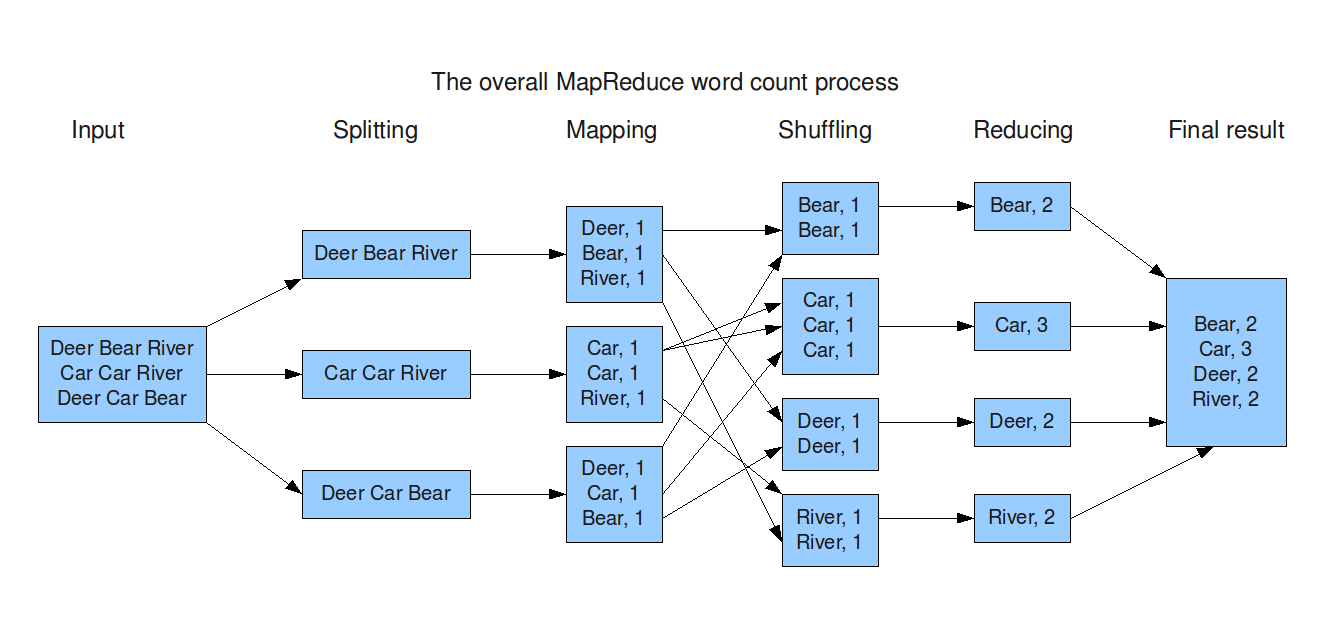
\includegraphics[scale=0.4]{img/archi.png}
\end{center}

\subsection{Architecture simple}
\subsubsection{Détail des différentes phases}
\paragraph{Constitution du cluster \\ \\}

Nous avons accès aux machines du campus de Télécom Paris mais la problématique est de savoir quelle machine peut être utilisée. Dans un premier temps il est nécessaire pour nous d'être
connecté au VPN du campus afin de pouvoir communiquer via le protocole SSH avec les machines du réseau. Afin de constituer de manière automatique notre cluster nous avons 
scrappé le site \url{https://supervision.enst.fr/tp/} (accessible uniquement via VPN) afin de récupérer la liste des machines actuellement allumées sur le réseau. Grâce à cette information nous
pouvons choisir un nombre de machine arbitraire sur lesquelles nous effectuons un test de connexion ssh afin de valider leur disponibilité.


Finalement, en exécutant le script \texttt{update\_cluster.py n} nous mettons automatiquement à jour un fichier 'machines.txt' contenant n noms de machines à notre disposition.


\paragraph{Splitting \\ \\}

Afin de séparer proprement notre texte d'entrée en plusieurs sous-fichiers nous avons utilisé la fonction \texttt{split} inhérente à Linux. Cette méthode nous permet
de subdiviser un fichier selon différents critères comme la taille maximale des sous fichiers. Le problème de cette méthode réside dans le fait que le découpage se fait 
en fonction des bits du fichier, et ne considère donc pas l'encodage de notre fichier. Cela mène à des erreurs dans les fichiers résultants ou à des mots coupés en deux. 
Nous avons donc choisi de compter le nombre de ligne de notre fichier avec la fonction \texttt{wc -l} de Linux nous permettant de compter très rapidemment le 
nombre de lignes du fichier. Ainsi, nous avons choisi de faire un découpage par lignes de notre fichier grâce à \texttt{split -l n} qui imposent aux sous fichiers de contenir n lignes au maximum.

Suite à cette phase, le master enverra les splits sur les différentes machines du cluster.
\paragraph{Mapping \\ \\}

Le master exécute de manière parallèle (en utilisant le maximum de coeur de la machine) les différentes phases de mapping sur toutes 
les machines du cluster. Chacune d'elle est chargée de lire les splits et d'écrire chaque mot dans un nouveau fichier suivi du chiffre 1 (ex: "maison" $\rightarrow$ "maison 1"). 
Cette phase prépare la phase de comptage ultérieure.

\paragraph{Shuffling \\ \\}

Toujours de manière parallélisée, le master va exécuter la phase de shuffle sur chaque slave. Ils calculent un hash unique associé à chaque mot qu'ils ont rencontré afin de pouvoir lui attribuer une machine sur laquelle il va être traité en finalité. Chaque mot différent sera stocké
dans un seul fichier qui sera ensuite attribué à une des machines du cluster. Finalement, après cette étape, toutes les occurences d'un même se retrouveront
stockées sur une même machine qui pourra faire le décompte final.

\paragraph{Reducing \\ \\}

Enfin, le master exécute de manière parallélisée l'étape de Reducing sur les slaves. Ils sont alors chargés de compter les occurences de chaque mot qui leur a été attribué (grâce au hash caculé précédemment).


\subsubsection{Résultats}

Nous allons comparer nos résultats pour le fichier "input.txt" de démonstration ne contenant que 3 lignes ainsi que le fichier \textit{forestier} qui est le deuxième plus petit de notre liste. Nous avons suivi l'exemple initial qui était de créer un cluster
de 3 machines sur lesquelles nous allions envoyer nos 3 spits. Dans ce contexte nous avons obtenu les résultats suivants:
\begin{table}[h!]
    \begin{center}
        \begin{tabular}{| l || c | c | c | c | c || c |}
            \hline			
              \textbf{Nom du fichier} & \textbf{Split + Déploiement} & \textbf{Map} & \textbf{Shuffle} & \textbf{Reduce} & \textbf{Total} & \textbf{Séquentiel}\\ \hline
              Input.txt & 1266 & 420 & 2042 & 438 & 5215 & \textbf{0.27}\\ \hline 
              Forestier.txt & 1300 & 467 & 33881 & 450 & 36898 & \textbf{0.64}\\ \hline
        \end{tabular}
    \end{center}
    \caption{Comparaison du temps d'exécution (en ms) du wordcount distribué et du wordcount séquentiel}
\end{table}

On remarque que notre programme réparti est bien plus lent que notre programme séquentiel. Nous pouvons imaginer que pour des fichiers plus volumineux notre programme réparti serait plus performant 
cependant notre implémentation fait que le temps de shuffle est proportionelle au nombre de mots différents car nous créons un fichier différent pour chaque mot que nous envoyons ensuite sur une autre machine
via le protocole SSH. Nous devons faire en sorte de modifier notre programme pour qu'il prenne en compte des plus gros fichiers.

Il est a noté que toutes les tâches sont lancées en parallèle, donc pour un programme MapReduce séquentiel les résultats auraient été encore plus désastreux.
\subsubsection{Limites}

Notre programme fonctionne mais devient très lent pour de gros fichiers, or nous devrions justement voir une améliration par rapport à la version séquentielle pour de gros fichiers.
Cette sous-performance est dû à plusieurs choses:
\begin{itemize}
    \item Lors de notre phase de Shuffle, nous créons un fichier différent par mot ce qui a pour effet de nous faire perdre beaucoup de temps en I/O puis en temps de transfert sur le réseau par la suite.
    \item La phase de Deploy est très longue car l'exécution s'effectue depuis un ordinateur qui est hors du cluster (mon ordinateur personnel). De fait la qualité du réseau n'est pas optimale.
    \item Les phases de parallélisation opérées par le master sont limitées par le nombre de coeurs du processeur de la machine qui l'exécute. Mon ordinateur n'en possède que 2 donc les gains sont très minimes.
\end{itemize}


\subsection{Architecture optimisée}
\subsubsection{Détail des modifications apportées}
\textbf{Modification du shuffle}: Afin de limiter le nombre de fichier créés et ainsi limiter l'I/O nous avons choisi une stratégie différentes pour le shuffle. Initialement,
nous créions un fichier par mot différent rencontré. Maintenant, nous créons un fichier par machine que nous remplissons de tous les mots attribués à cette dernière. De fait, nous créons moins de fichier différents et 
nous ouvrons/fermons moins de fichier ce qui a pour effet de grandement améliorer les performances et de réduire la charge du réseau lors du transfert. Enfin, nous avons parallélisé l'écriture et l'envoie des différents 
fichiers ce qui a pour effet d'accélérer encore plus cette phase.


\textbf{Modification de l'interface entre le cluster et notre machine}: Nous avons choisi de rajouter une nouvelle machine \textit{Edge} à notre cluster
qui va servir d'interface entre notre machine et le cluster. Cette machine sert à orchestrer tout le lancement du MapReduce (splitting, déploiement, map, shuffle et reduce).
Cette modification améliore notre programme sur plusieurs points:
\begin{itemize}
    \item Le \textbf{deploy} était initialement très lent car les données devait transiter de ma machine jusqu'au réseau de Télécom ce qui représentait un très gros goulot d'étranglement. Maitenant,
    la donnée transite uniquement au sein du réseau de Télécom (réseau filaire très rapide) ce qui permet d'augmenter considérablement le débit.
    \item Les machines de Télécom possèdent 12 coeurs, ce qui permet de faire tourner 12 processus en simultané. Le lancement des phases de map, shuffle et reduce se fait par appel parallèle donc pour un cluster de 12 machines
    les exécutions peuvent se faire simultanément ce qui a encore pour effet d'accélérer le traitement.
\end{itemize}

Cette modification induit plusieurs nouveautés dans notre code. Nous avons ajouté un fichier \texttt{master.txt} qui contient le nom de la machine maître sur laquelle
nous allons copier les données voulues ainsi que les fichiers slave, master, clean, deploy. Toutes les commandes vont être lancé à partir de cette nouvelle machine. Pour faciliter
la communication avec ce \textit{Edge node} nous avons implémenté un utilitaire \texttt{supervisor.py} permettant de contrôler facilement les exécutions (voir dernière section pour plus d'informations).

\textbf{Nombre de splits et de noeuds}: Afin d'optimiser au maximum les performances de notre cluster nous avons choisi d'utiliser un cluster de \textbf{12 machines} afin de correspondre au nombre de coeurs
de notre master. Toutes les commandes parallèles peuvent alors être lancées en même temps sur tous les slaves. De même, nous avons choisi de diviser nos données en 12 (Note: nous aurions préféré diviser les fichiers
selon une taille de split maximale mais comme cité plus haut cette méthode entraîne des soucis).
\subsubsection{Résultats}

Nous avons effectué les tests sur un cluster de 12 machines slaves et une machine edge (master). Nous avons obtenu les résultats suivants:
\begin{table}[h!]
    \begin{center}
        \begin{tabular}{| l || c | c | c | c | c || c |}
            \hline			
              \textbf{Nom du fichier} & \textbf{Split + Déploiement} & \textbf{Map} & \textbf{Shuffle} & \textbf{Reduce} & \textbf{Total} & \textbf{Séquentiel}\\ \hline
              Déontologie.txt & 1162 & 451 & 1635 & 431 & 3679 & \textbf{2.00}\\ \hline
              Domaine.txt & 1262 & 452 & 1635 & 431 & 3780 & \textbf{10.28}\\ \hline
              Santé.txt & 1701 & 524 & 3240 & 413 & 5878 & \textbf{1206}\\ \hline
              Fichier 390 Mo & 5315 & 1552 & 8435 & 917 & \textbf{16219} & 41416\\ \hline
        \end{tabular}
    \end{center}
    \caption{Comparaison du temps d'exécution (en ms) du wordcount distribué (version améliorée) et du wordcount séquentiel}
\end{table}


On remarque que notre nouvelle architecture est beaucoup plus performante que la précédente, elle réussi même à battre le programme séquentiel pour le 
fichier de 390 Mo. La résolution des problèmes évoqués ci-dessus a donc bien permis de gérer le cas des gros fichiers, cependant pour les petits fichiers cette architecture n'est pas 
adaptée car nous avons un coût en temps de réseau qui est constant (d'où les valeurs quasi similaire pour les fichiers Domaine et Déontologie). Ce temps est supérieur au temps d'exécution du programme séquentiel
donc il doit y avoir un taille limite de fichier pour laquelle le cluster est plus efficace. Ci-dessous nous présentons un graphique de l'évolution du temps de traitement pour les programmes séquentiels et le cluster:


Il est à noter que les résultats obtenus dépendent du cluster utilisé et de l'heure d'utilisation. Le processus peut être plus lent ou plus rapide que le résultat reporté.
\begin{center}
    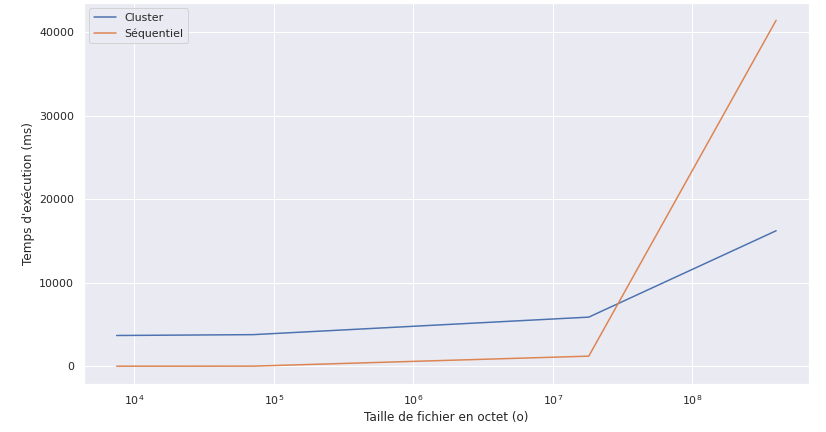
\includegraphics[scale=0.5]{img/graph.png}
\end{center}


On voit bien sur ce graphe que le temps d'exécution du programme séquentiel augmente très fortement avec la taille des fichiers alors que le programme déployé
sur un cluster gère assez bien des gros fichiers. Finalement, le paradigme MapReduce répond à sa promesse et nous permet d'améliorer le traitement des gros fichiers.

\subsubsection{Limites}

Notre programme n'est pas très robuste à l'heure actuelle c'est à dire qu'il ne gère pas les cas complexes ou les pannes. Plus précisemment, 
nous rencontrons deux principaux problèmes:
\begin{itemize}
    \item Lorsqu'une tâche échoue sur une machine, notre programme ne gère pas cet arrêt et le calcul continu mais les résultats sont faussés.
    \item Si le nombre de split est inférieur au nombre de machines disponibles dans notre cluster, il y a une erreur car les fonctions map, shuffle et reduce
    sont appelées sur toutes les machines du cluster et non pas seulement sur les machines sur lesquelles les splits ont été exporté.
\end{itemize}

\subsection{Architecture robuste}
\subsubsection{Détails des modifications apportées}
Nous avons modifié notre implémentation afin de résoudre les deux problèmes évoqués ci-dessus:

\begin{itemize}
    \item \textbf{Nombre de machine \& Nombre de splits}: pour régler ce problème nous avons créé un nouveau fichier \texttt{used\_machines.txt} qui se partage sur toutes les machines utilisées dans le cluster. 
    Ce fichier contient la liste des machines qui sont actuellement en train de calculer (les machines sur lesquelles un split a été déployé). Cette nouvelle liste nous permet de gérer tout type de fichier quelle que soit la taille du fichier d'entrée.
    \item \textbf{Gestion des pannes}: afin de conserver une trace de toutes les erreurs qui sont arrivées pendant l'exécution, le master rempli des fichiers \texttt{map.error}, \texttt{shuffle.error}, \texttt{reduce.error} lors des appels parallèles en y inscrivant le nom de la machine qui a fait défaut. 
    Ces écritures parallèles sur un même fichier s'effectuent grâce l'utilisation d'un blocage sur le fichier lorsque qu'un processus l'utilise. Avant chaque finalisation d'étape, notre programme vérifie le contenu de ces fichiers et si une machine a fait défaut sur une des tâches, il la supprime du fichier
    \texttt{used\_machines.txt} et relance entièrement le job MapReduce (il faudrait pouvoir relancer le processus à partir d'une étape en particulier si possible). Dans ce cas, nous ne changons pas le nombre de splits mais une machine récupère la charge de travail de la machine down.
\end{itemize}

Afin de finaliser notre programme pour le rendre utilisable facilement nous avons opéré d'autres modifications:
\begin{itemize}
    \item Nous avons aussi permis au master d'afficher les résulats triés en sortie du MapReduce. Pour se faire nous devons choisir un nombre $n$ de valeurs à remonter, ainsi chacun des slaves va trier toutes ses valeurs et envoyer les $n$ premières sur le master.
    Le master doit ensuite trier $n * n_machines$ valeurs et afficher les $n$ premiers. Cette méthode nous permet de retourner le résulat sans avoir à faire un Reduce entier sur le master.
    \item Nous avons fait en sorte que les fichiers créé sur une node lors d'une instance de MapReduce n'influent pas sur les résultats du suivant. Pour ce faire on opère une étape de nettoyage des dossiers créé avant d'effectuer le Map.
    \item Nous avons amélioré la remontée des pannes au master en gérant et en remontant les exceptions à toutes les étapes.
    \item  Enfin, nous avons simplifié l'utilisation du programme (cf dernière section) et géré les couleurs dans le terminal pour plus de visibilité.
\end{itemize}

Toutes ces modifications ont été référencées proprement dans le code qui a d'ailleurs été entièrement commenté et rendu lisible.

\section{Utilisation du programme}
Afin d'utiliser correctement notre programme, l'utilisateur a besoin de \textbf{4 commandes} différentes:
\begin{itemize}
    \item \texttt{python3 update\_cluster n}: permet de récupérer une liste de machines allumées et réactives servant de slave et master.
    \begin{center}
        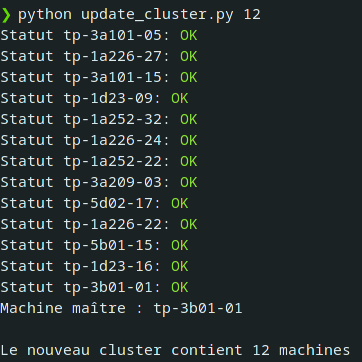
\includegraphics[scale=0.5]{img/update.png}
    \end{center}    
    \item \texttt{python3 supervisor.py load path\_to\_data}: permet de charger notre donnée sur le master (edge node) de notre cluster.
    \begin{center}
        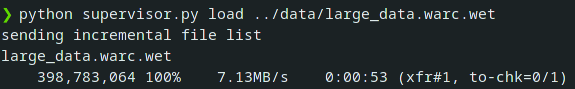
\includegraphics[scale=0.5]{img/load.png}
    \end{center}    
    \item \texttt{python3 supervisor.py run}: permet de mettre à jour les fichiers sur le master et les slaves, puis lance le process mapreduce et affiche les résulats (10 premiers par défaut).
    \begin{center}
        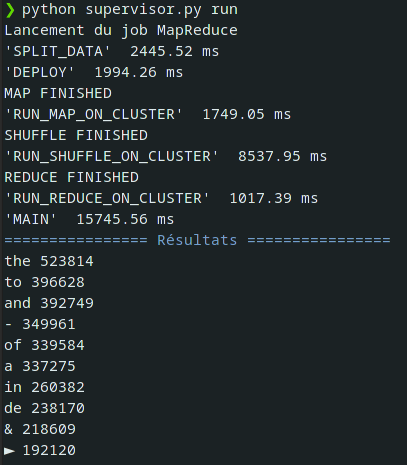
\includegraphics[scale=0.5]{img/mapreduce.png}
    \end{center}
    \item \texttt{python3 supervisor.py clean}: permet de nettoyer tout le cluster (master et slaves).
    \begin{center}
        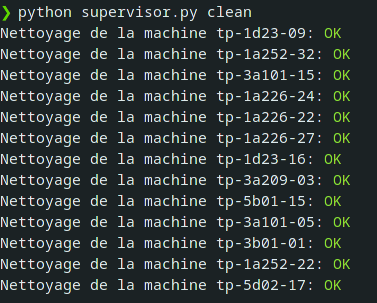
\includegraphics[scale=0.5]{img/clean.png}
    \end{center}
     
\end{itemize}

\end{document}

